\documentclass{article}
\PassOptionsToPackage{numbers,sort&compress}{natbib}
\usepackage[dblblindworkshop]{shared/neurips_2026}
\workshoptitle{RoboPAD: Post-Training Adaptation of Robot Foundation Models}
\usepackage[T1]{fontenc}
\usepackage[utf8]{inputenc}
\usepackage{microtype}
\usepackage{booktabs}
\usepackage{graphicx}
\usepackage{amsmath,amssymb}
\usepackage{enumitem}
\usepackage{siunitx}
\usepackage[hidelinks]{hyperref}
\usepackage{placeins}
\title{Refinement versus Refresh:\\
Compute Allocation for Closed-Loop Robot Policies}
\author{Anonymous Authors}
\begin{document}
\maketitle

\begin{abstract}
Robot policies increasingly spend substantial inference compute refining actions
before execution, but it is unclear whether this extra computation improves
closed-loop control. We report an empirical study in progress of this deployment
trade-off in one frozen SmolVLA policy, combining a paired, 12-configuration
discovery study with a prespecified comparison on eight LIBERO tasks excluded
from configuration selection. At a fixed two-action prefix, reducing denoising
from five steps to two increases success from 122/160 to 139/160: a paired
difference of 10.6 percentage points with a task-conditional, descriptive 95\%
interval of 4.4--16.9 points.
The observed direction agrees with the frozen prediction of 4.0 points, but its
magnitude is larger. Relative to the same comparator, reference-calibrated dense
arithmetic is 5.9\% lower per control step; mean arithmetic per attempt is 41.1
versus 48.7 TFLOPs, including failures. The 480-attempt discovery study varies
both refinement and execution prefix, and full-generation calibration assigns
82.1\% of native counted arithmetic to denoising-independent work. A simple
cost-aware rule matches the fitted response model's configuration choices at
three budget ceilings. For this checkpoint, the separate-task comparison shows
that reducing refinement can improve closed-loop success while lowering
computation. These findings motivate further study of when additional refinement
improves quality and when computation is better spent on more frequent
observation-conditioned predictions.
\end{abstract}

\section{Introduction}

A robot policy can reduce inference work in two ways: spend less computation
refining each action prediction, or execute more actions before requesting a
new prediction. These interventions affect behavior differently. Reduced
refinement changes the prediction itself; longer execution prefixes delay
observation-conditioned revision and expose later positions of the predicted
action sequence. Their relative value should therefore be evaluated through
closed-loop outcomes under a common resource constraint.

We ask: \emph{given a fixed inference budget, how should a robot divide
computation between prediction refinement and observation-conditioned refresh?}
A broader objective is to use a limited calibration study to guide deployment
on tasks excluded from selection. Here we test whether a discovery-selected
reduction in denoising improves success at a fixed execution prefix. This
comparison tests transfer of a configuration choice; the broader allocation
relationship remains open.

We vary denoising steps $d$ and executed prefix $h$ for one frozen SmolVLA
checkpoint \cite{smolvla}. The predicted chunk remains 50 actions. Our
12-configuration study measures both task success and resource use. A fitted
response model and a simple cost-aware rule nominate the same configurations
at three compute-rate ceilings. At the primary ceiling, ordinary empirical
selection agrees as well. The independent comparison favors their shared choice:
two denoising steps produce 139/160 successes versus 122/160 for five steps at
$h=2$, with lower reference-calibrated arithmetic.

The budget coordinate is consequential. Neural work performed once per
generation persists when denoising is reduced. In our calibration, all work
independent of denoising accounts for 82.1\% of native dense arithmetic, making $d/h$ a poor
proxy for compute rate. Meanwhile, changing a configuration changes trajectories
and episode duration, so equal rate ceilings do not imply equal realized
episode expenditure. We report both coordinates.

This paper makes three contributions:
\begin{itemize}[leftmargin=*,nosep]
    \item a paired 12-configuration study of refinement and execution prefix,
    reporting both compute rate and realized episode expenditure;
    \item a full-generation calibration that measures denoising-independent
    per-generation arithmetic under an explicit operation boundary; and
    \item a prespecified, separate-task comparison in which lower denoising
    improves observed success and reduces reference-calibrated computation at
    a fixed prefix.
\end{itemize}
The evidence concerns one frozen policy, four discovery tasks, and eight
transfer tasks excluded from configuration selection. It combines a finite
deployment study with a completed, prespecified primary task-transfer
comparison. Together, these measurements show why deployment settings should
be selected using closed-loop quality as well as computation: additional
refinement can consume more resources while reducing observed success.

\section{Related Work}

Resource-allocation studies motivate evaluating configurations across explicit
budgets. Chinchilla studies model-size and training-data allocation
\cite{chinchilla}; embodied scaling studies consider world modeling, behavior
cloning, and closed-loop forecasting and planning
\cite{pearcescaling,motionscaling}. Our comparison instead varies deployment
refinement and execution prefix within a fixed policy. Work distinguishing
FLOP-optimal from elapsed- or monetary-cost-optimal allocation
\cite{beyondchinchilla} also motivates retaining separate resource coordinates.

VLA-Perf characterizes inference performance across denoising, chunk size,
asynchronous execution, and hardware/runtime choices \cite{vlaperf}.
SmolVLA studies asynchronous inference and robot behavior \cite{smolvla}.
Here predicted chunk size remains fixed, while executed prefix changes; task
success is measured alongside computation. RoboMonkey studies test-time sampling
and action verification \cite{robomonkey}, an adjacent allocation axis that
would require counting candidate generation and verification costs.

Adaptive VLA scheduling is directly related. DVAC uses denoising-derived action
variance to choose an execution prefix before replanning \cite{dvac}.
ElegantVLA schedules vision--language recomputation or reuse together with action
denoising modes \cite{elegantvla}. Our study instead compares fixed configurations
under explicit arithmetic ceilings and freezes a separate-task denoising
comparison. It neither introduces an adaptive scheduler nor establishes an
advantage over these methods; their reported speedups have different policies,
hardware, and measurement boundaries.

\section{Experimental Design}
\label{sec:method}

\subsection{Compute-rate constraint}

Let $F_{\mathrm{gen}}(d)$ denote reference-calibrated neural arithmetic for a full
action-chunk generation at denoising setting $d$. For complete execution prefixes, the nominal
compute rate per simulated control step is
\[
 b(h,d)=\frac{F_{\mathrm{gen}}(d)}{h}.
\]
For a candidate set $\mathcal C$ and budget ceiling $B$, the allocation target is
\begin{equation}
 (h^\star,d^\star)(B)\in
 \arg\max_{(h,d)\in\mathcal C:\,b(h,d)\le B}
 p_{\mathrm{success}}(h,d).
 \label{eq:allocation}
\end{equation}
A configuration need not exhaust the ceiling. This is a deployment compute-rate
constraint for a fixed checkpoint, rather than a training-plus-deployment
objective.

We distinguish this rate from total arithmetic per attempted episode. If attempt
$e$ executes $T_e$ actions, its generated-chunk expenditure is
\begin{equation}
 C_e=\left\lceil T_e/h\right\rceil F_{\mathrm{gen}}(d).
 \label{eq:episode-cost}
\end{equation}
The final generated chunk is charged even if only part of its execution prefix
is used. All-attempt means include unsuccessful episodes. Different trajectories
and termination times can therefore change expenditure at the same nominal rate.
FLOPs, host elapsed time, and CUDA-stream time retain separate units and
measurement boundaries.

\subsection{Policy, tasks, and pairing}

We evaluate the public \texttt{HuggingFaceVLA/smolvla\_libero} checkpoint on LIBERO
\cite{libero}, with
\[
 h\in\{1,2,5\}, \qquad d\in\{2,5,10,20\}.
\]
Native deployment is $(h,d)=(1,10)$. We hold weights, predicted chunk length,
sensors, preprocessing, action normalization, control period, and episode
horizon fixed. Changing $h$ selects how many successive predicted actions are
executed before the next generation.

The design crosses Spatial tasks 5--8 with five initial states and two policy
seeds: 40 task--state--seed identities, each evaluated under all 12 conditions,
for 480 attempts. Tasks 5 and 6 overlap the pilot; tasks 7 and 8 were selected
before observing their outcomes in this study. All conditions, including native,
are evaluated within the same measurement study. Their order is randomized
within each paired identity.

Initial simulator states and observations match across conditions. Policy noise
is keyed by task, state, seed, and simulation tick, so changing generation
frequency uses the same random stream across conditions. Action-dispatch,
generation, denoising, and outcome records are reconciled independently across
software boundaries (\hyperref[app:verification]{Appendix~\ref{app:calibration}}).

\subsection{Cost calibration and uncertainty}

Complete-generation profiling counts matrix products, convolutions, and
attention across vision, language prefill, and the action expert, using two
FLOPs per multiply-add. Embedding lookups, normalization, activations,
elementwise arithmetic, and external preprocessing are excluded. We therefore
refer to \emph{dense neural arithmetic}, not an exact count of every scalar
operation. Calibration uses one real development observation and fixed tensor
shapes; its protocol is detailed in Appendix~\ref{app:calibration}.

The profiled batch contains one sample, two $3\times360\times360$ image tensors,
an eight-dimensional state tensor, and language-token and attention-mask tensors
of length 20. The checkpoint exposes seven-dimensional actions and generates a
50-action chunk. Evaluation fixes batch size, image preprocessing, state/action
dimensions, and chunk size. The tokenizer pads language only to the longest
sequence in a batch. Reconstructing the declared task strings with the pinned
tokenizer gives 15--17 tokens for discovery and 5--12 for transfer, versus 20
in calibration. We profile these distinct lengths for $d\in\{2,5,10\}$ and
test eligibility against the original absolute ceilings; Section~\ref{sec:results}
reports the result and Appendix~\ref{app:shape-audit} gives the counts.

The actual solver timesteps and a constant-field integration check verify that
each $d$ traverses the full interval from 1 to 0. Reducing $d$ changes the
discretization, rather than truncating the native solver. The calibration
includes $d=3,8$ for candidate configurations whose task success is not measured
during discovery.

All measurements use an RTX 4060 Ti. Five-second process samples show no
unrelated CUDA compute process during calibration, discovery, or the initially
scheduled transfer phase; display processes remain. Process samples were not
retained for priority completion, so transfer rollout times are descriptive.
Host and CUDA-stream generation intervals are measured separately
from the outer synchronous rollout interval. Warm-up is excluded from these
rollout measurements.

Task success is averaged over both policy seeds within each state, then over
states and tasks with equal task weights. Figure~\ref{fig:frontier} reports
descriptive 95\% intervals from 20,000 bootstrap draws, resampling states within
each of the four fixed tasks while preserving both seeds and all configurations.
These intervals are descriptive and conditional on the four discovery tasks.

\section{Discovery Results}

\subsection{Full-generation work is dominated by the fixed component}
\label{sec:results}

The measured arithmetic counts satisfy, to rounding,
\[
 F_{\mathrm{gen}}(d)\simeq 527.108+11.457d\quad\text{GFLOPs}
\]
at all six calibrated denoising settings. Native generation costs 641.675 GFLOPs,
of which 82.1\% is independent of $d$. Halving denoising from ten to five saves
8.9\% of counted generation work; reducing it to two saves 14.3\%.

Across the evaluated language lengths, generation arithmetic increases with
length and no reported transfer configuration changes eligibility under the
fixed absolute ceilings. This includes the boundary configuration $(2,10)$ at
half-native rate. Eligibility is unchanged; reference-calibrated counts remain
distinct from the lower task-shape-specific counts.

The budget ceilings are prespecified at $0.25$, $0.50$, and $1.00$ times native
rate. Eligibility uses the measured per-$d$ values rather than the rounded
affine expression. For example, $(1,2)$ costs 0.857 times native rate and remains
ineligible at half-native budget, whereas $(2,2)$ costs 0.429 times native.
Frequent observation-conditioned refresh therefore carries substantial work
even with few denoising steps.

Equivalently, the measured cost model gives
\[
 \frac{b(h,d)}{b_{\mathrm{native}}}
 \simeq \frac{0.821+0.179(d/10)}{h}.
\]
The work independent of denoising alone exceeds a half-native budget at $h=1$.
This is an implementation-specific arithmetic floor under the declared input
shape and counting boundary, not a universal VLA scaling relationship.

Within the discovery grid, no $h=1$ configuration is eligible at half-native
budget, and no $h\leq2$ configuration is eligible at quarter-native budget.
Thus a shift toward longer prefixes at tighter ceilings is partly imposed by
feasibility. Evidence for a useful allocation predictor must concern its choice
among eligible alternatives, not this shift alone.

\subsection{The quality--compute relationship}

Native $(1,10)$ succeeds in 25/40 attempts. The highest observed success is 28/40
for $(1,5)$; $(1,2)$ and $(2,2)$ each succeed in 26/40. At $h=5$, successes are
21, 18, 16, and 14 out of 40 as $d$ increases from 2 to 20.
Figure~\ref{fig:frontier} shows every configuration, and
Table~\ref{tab:discovery-grid} reports task-level counts. The point estimates
do not justify imposing monotonic improvement with denoising.

\begin{figure}[t]
\centering
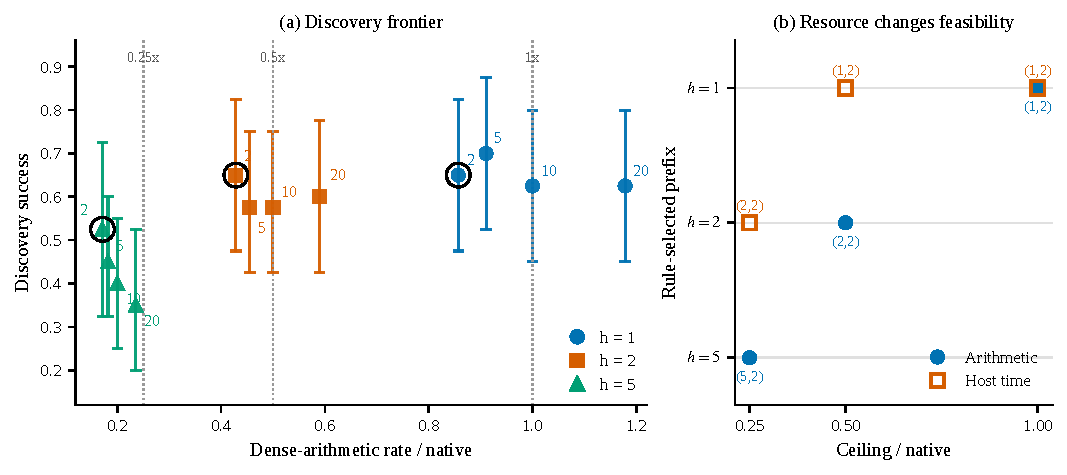
\includegraphics[width=\linewidth]{experiments/executed/refinement_refresh_final_001/paper_analysis/discovery_frontier.pdf}
\caption{Discovery quality and resource-dependent feasibility. (a) Point labels
give $d$ and marker shapes give $h$; each configuration has 40 attempts. Bars are
descriptive 95\% state-bootstrap intervals conditional on the four tasks. Dotted
lines mark arithmetic ceilings and rings identify model-selected configurations.
(b) The same minimum-denoising, shortest-feasible-prefix rule selects different
prefixes under separately normalized arithmetic and fixed-input host-time ceilings.
Thus the resource definition changes feasible refresh schedules before quality
selection; panel (b) does not identify quality optima.}
\label{fig:frontier}
\end{figure}

These results distinguish expenditure from quality. Relative to native, $(2,2)$
has a lower nominal rate and a similar observed success count, but the small
paired sample does not certify equivalent quality. At $h=5$, additional
refinement does not recover the observed success of shorter prefixes on this
task set. The comparison does not identify a universal optimum: changing $h$
also changes the action positions executed.

Arithmetic savings and elapsed savings differ. Mean rollout time is 111.9 seconds
per attempt for native deployment, 61.8 seconds for $(1,5)$, and 21.8 seconds for
$(2,2)$. Their mean generated-chunk expenditures are 109.6, 91.7, and 45.0 TFLOPs,
respectively. These are observed all-attempt means under the same task allocation;
they include different trajectories and outcomes. The full resource table is
provided in Appendix~\ref{app:calibration}.

There is also an ordering reversal: $(1,5)$ uses more arithmetic per attempt
than $(2,20)$ (91.7 versus 67.8 TFLOPs), but less rollout time (61.8 versus
107.8 seconds). These means include different trajectories. On a fixed input,
reducing $d$ from 10 to 5 lowers mean generation host time from 629.6 to
374.3 ms (40.5\%), despite only 8.9\% less counted arithmetic. The calibration
therefore also separates arithmetic savings from elapsed savings without
trajectory differences. It does not resolve their component-level cause
(Appendix~\ref{app:fixed-timing}). A FLOP-constrained choice is not necessarily
a latency- or throughput-optimal choice.

As a descriptive sensitivity analysis, define calibrated host-time rate
$b_T(h,d)=\overline{T}_{\mathrm{gen}}(d)/h$, the amortized fixed-input generation
time per simulated control step, and normalize it by native host-time rate.
For $(1,2)$, $(2,2)$, and $(5,2)$, the normalized arithmetic rates are
0.857, 0.429, and 0.171, while the normalized host-time rates are 0.346, 0.173,
and 0.069. Consequently, $(1,2)$ is ineligible at a half-native arithmetic
ceiling but eligible at a separately normalized half-native host-time ceiling.
Figure~\ref{fig:frontier}(b) shows the resulting choices at all three ceilings.
These resource constraints admit different refresh schedules; the choices do
not establish quality optima. The frozen experiment remains arithmetic-based.

\FloatBarrier
\subsection{Response models and frozen predictions}
\label{sec:prediction}

We compare two logistic response-model families. A compute-only model uses a
quadratic in log normalized rate. An allocation model uses $\log h$,
$\log(d/10)$, both squared terms, and their interaction. Each family is fitted
with ridge penalty 1 or 10. Leave-one-task-out log loss selects the model, which
is then refitted on the discovery set. No individual seed repeat is held out
while another repeat from the same task remains in training.

The candidate set is $h\in\{1,2,3,5\}$ crossed with $d\in\{2,3,5,8,10,20\}$:
the 12 discovery configurations and 12 untested configurations. Their calibrated costs determine
eligibility; the fitted model selects the highest predicted success under each
ceiling. Ties favor lower compute, then lexicographic order.

\begin{table}[htbp]
\centering\small
\setlength{\tabcolsep}{2.4pt}
\caption{Discovery-based selector choices and frozen allocation predictions.
The empirical selector uses the measured grid; other selectors use the declared
candidate set. The simple rule exactly matches the learned choices. Selected
rate/native is the learned recommendation's arithmetic rate; comparator and gap
define the frozen transfer tests. The bold half-native row is primary.
}
\label{tab:selectors}
\label{tab:predictions}
\begin{tabular}{@{}rccccrrr@{}}
\toprule
& \multicolumn{4}{c}{Selector choice $(h,d)$} & \multicolumn{3}{c}{Frozen prediction}\\
\cmidrule(lr){2-5}\cmidrule(l){6-8}
$B/B_{\rm nat}$ & Learned & Simple & Empirical & Compute-only & Comparator & \shortstack{Selected\\rate/native} & Gap (pp)\\
\midrule
0.25 & $(5,2)$ & $(5,2)$ & $(5,2)$ & $(5,20)$ & $(5,5)$ & 0.171 & $+6.5$\\
\textbf{0.50} & $\mathbf{(2,2)}$ & $\mathbf{(2,2)}$ & $\mathbf{(2,2)}$ & $\mathbf{(2,10)}$ & $\mathbf{(2,5)}$ & \textbf{0.429} & $\mathbf{+4.0}$\\
1.00 & $(1,2)$ & $(1,2)$ & $(1,5)$ & $(1,10)$ & $(1,5)$ & 0.857 & $+2.2$\\
\bottomrule
\end{tabular}
\end{table}

The simple rule minimizes denoising count, then chooses the shortest feasible
prefix. It reproduces every learned recommendation (Table~\ref{tab:selectors});
transfer outcomes cannot distinguish these selectors at the tested budgets.
The compute-only choices use the original ridge-10 fit. Its quarter- and
half-budget choices are absent from the transfer plan, so this evaluation
cannot compare those decisions on transfer tasks.

The selected allocation model has log loss 0.7048, compared with 0.7067 for the
best compute-only model. This small difference provides no evidence of an added
predictive advantage. Under the same mean natural-log binary cross-entropy,
constant $p=0.5$ scores 0.6931 and an intercept-only model fitted separately on
each training fold scores 0.7170. The response-model probabilities should
therefore not be read as calibrated task-transfer forecasts. The primary test
evaluates a recommendation shared with simpler selectors, so it does not
establish an additional benefit from model-based ranking.

\FloatBarrier

\section{Primary Task-Transfer Evaluation}
\label{sec:transfer}

\subsection{Protocol and evaluation sample}

At the primary half-native ceiling, the recommendation $(2,2)$ has the highest
eligible discovery success. Its frozen comparator, $(2,5)$, ties with $(2,10)$
for the highest success among distinct eligible alternatives; the lower-cost
tie-break selects $(2,5)$. Both are existing grid points, so
the test concerns transfer across tasks rather than extrapolation to an untested
configuration. Table~\ref{tab:predictions} retains the frozen secondary
predictions for transparency; only the primary pair is reported here.

The primary protocol uses Object and Goal tasks 5--8, states 20--29,
and seeds 3000 and 3001, giving 160 attempts per configuration across
80 task--state blocks. The selection and predicted difference were fixed before
transfer evaluation. These tasks were excluded from configuration selection;
prior exposure during unrelated development is not assessed. Both configurations
cover every originally planned identity. The allocation was chosen for task and
state coverage; no quality margin was prespecified.

\subsection{Primary result}

\begin{table}[htbp]
\centering\small
\setlength{\tabcolsep}{5pt}
\caption{Primary transfer comparison on eight tasks excluded from selection.
Ref.\ rate/native is $F_{\mathrm{gen}}(d)/(hF_{\mathrm{gen}}(10))$.
Ref.\ TFLOPs multiply recorded generation counts by the original length-20
calibration. Costs average all attempts, including failures. The descriptive
95\% interval uses 20,000 bootstrap draws of paired states within each task,
retaining both seeds. Rollout times are descriptive observed means: process
monitoring was not retained during priority completion.}
\label{tab:primary-transfer}
\begin{tabular}{@{}lcS[table-format=1.3]S[table-format=2.1]S[table-format=2.1]@{}}
\toprule
Configuration & Success & {Ref. rate/native} & {Ref. TFLOPs/attempt} & {Observed rollout s}\\
\midrule
Selected $(2,2)$ & 139/160 (86.9\%) & 0.429 & 41.1 & 19.0\\
Comparator $(2,5)$ & 122/160 (76.3\%) & 0.455 & 48.7 & 34.3\\
\midrule
\multicolumn{2}{@{}l}{Frozen predicted gap} & \multicolumn{3}{l}{\hspace{3pt}$+4.0$ pp}\\
\multicolumn{2}{@{}l}{Observed paired gap} & \multicolumn{3}{l}{\hspace{3pt}$+10.6$ pp $[+4.4,+16.9]$}\\
\bottomrule
\end{tabular}
\end{table}

The selected configuration succeeds in 86.9\% of attempts, compared with 76.3\%
for the comparator. The observed paired difference is 10.6 percentage points,
6.6 points larger than the frozen prediction. Its descriptive interval excludes
zero under the declared task-conditional bootstrap. The direction therefore
agrees with the prospective prediction on tasks excluded from selection, although
the predicted magnitude understates the observed gap.

Both configurations satisfy the half-native ceiling. Reference-calibrated rates
are 275.0 GFLOPs per control step for $(2,2)$ and 292.2 for $(2,5)$, a 5.9\%
reduction distinct from realized episode expenditure (Table~\ref{tab:primary-transfer}).

\begin{table}[htbp]
\centering\small
\caption{Primary outcomes by task at $h=2$. Each condition has ten states and
two seeds per task. A win is a paired task--state--seed identity where only
$d=2$ succeeds; a loss is one where only $d=5$ succeeds. These joint counts
describe the observed pairs; uncertainty resamples states with both seeds
retained, not independent seed repeats.}
\label{tab:primary-tasks}
\begin{tabular}{@{}lrrrrr@{}}
\toprule
Task & Selected $d=2$ & Comparator $d=5$ & Gap (pp) & Wins & Losses\\
\midrule
Goal 5 & 16/20 & 14/20 & $+10.0$ & 4 & 2\\
Goal 6 & 18/20 & 15/20 & $+15.0$ & 3 & 0\\
Goal 7 & 19/20 & 18/20 & $+5.0$ & 1 & 0\\
Goal 8 & 18/20 & 14/20 & $+20.0$ & 5 & 1\\
Object 5 & 20/20 & 20/20 & $+0.0$ & 0 & 0\\
Object 6 & 20/20 & 17/20 & $+15.0$ & 3 & 0\\
Object 7 & 10/20 & 7/20 & $+15.0$ & 6 & 3\\
Object 8 & 18/20 & 17/20 & $+5.0$ & 2 & 1\\
\midrule
All tasks & 139/160 & 122/160 & $+10.6$ & 24 & 7\\
\bottomrule
\end{tabular}

\end{table}

The selected configuration has a higher success count on seven tasks and ties
on one (Table~\ref{tab:primary-tasks}). There are 24 paired wins and seven
losses. In a descriptive leave-one-task-out sensitivity analysis, the
equally weighted difference over the remaining seven tasks stays positive,
ranging from 9.3 to 12.1 percentage points. This post-outcome analysis does not
extend inference to a new task population. The supplementary paired records
retain all state and seed identities needed to reproduce the primary interval.

Mean episode length is 149.0 versus 166.3 control steps. All failures reach
the task horizon (21 versus 38); other attempts terminate successfully.
The 15.6\% reduction in mean reference-calibrated episode arithmetic therefore
includes changed trajectory lengths and termination, not just the 5.9\%
per-step saving. Appendix~\ref{app:primary-costs} gives paired expenditure
intervals. Observed rollout means remain descriptive rather than a controlled
physical-latency claim.

At half-native budget, the learned model, empirical discovery selector, and
simple rule all choose $(2,2)$. This result supports their shared configuration
choice against the frozen distinct comparator. At a fixed two-action prefix,
less refinement improves observed success while reducing arithmetic per control
step and per attempt. This separate-task result provides evidence that
deployment quality must be measured directly rather than inferred from sampler
effort. Comparing execution prefixes on separate tasks is the next step toward
testing the broader refinement--refresh allocation relationship.

\section{Discussion and Conclusion}

\paragraph{Limitations.}
The study covers one checkpoint, four discovery tasks, and eight transfer tasks
in simulation. Intervals condition on these tasks, and the fitted models have
only four task-level validation folds. The arithmetic boundary excludes several
operation classes; language lengths are audited, but image shape remains fixed.
Sampled process checks cannot exclude all hardware interference, and neither
nominal refresh interval nor simulator throughput establishes real-time
responsiveness. Longer prefixes change both observation freshness and executed
action positions. Two steps is the minimum tested denoising setting, not an
established lower limit; $d=1$ is untested. The mechanism behind the advantage
of coarser sampling, other policies, and broader allocation comparisons remain
open research questions.

Together, the results separate two deployment decisions: full-generation cost
determines which refresh schedules are feasible, while closed-loop outcomes
determine which feasible choice is useful. For this SmolVLA implementation,
the primary transfer result favors two over five denoising steps at $h=2$
under a half-native arithmetic ceiling: success increases by 10.6 percentage
points while reference-calibrated arithmetic per control step falls by 5.9\%.
A simple cost-aware rule makes the same choices as the fitted response model
at the tested ceilings. The practical implication is to evaluate refinement
settings against closed-loop quality, since additional sampler computation can
worsen both quality and expenditure. The next research stage is to test whether
limited calibration can guide choices between refinement and refresh across
execution prefixes, budgets, and policies.

\clearpage
\bibliographystyle{unsrtnat}
{\raggedright\bibliography{references}}
\clearpage
\appendix

\section{Detailed Outcomes and Resource Measurements}
\label{app:calibration}

{\raggedright
The checkpoint is \texttt{HuggingFaceVLA/smolvla\_libero}, revision
\texttt{6721902bc4d61e50a3bfdb11dfb4cb626f05d102}. Predicted chunk size is 50;
native execution uses $h=1,d=10$. Discovery uses Spatial tasks 5--8, initial
states 10--14, and policy seeds 2000 and 2001. The 20 task--state blocks
contain both seeds and all 12 configurations. Discovery bootstrap resampling uses
20,000 draws with analysis seed 20260913.\par}

\begin{table}[htbp]
\centering\small
\caption{Discovery successes on Spatial tasks 5--8. Each task contributes five
states and two seeds per configuration. Rate/native is
$F_{\mathrm{gen}}(d)/(hF_{\mathrm{gen}}(10))$, not realized episode cost.
The best observed count is 28/40 at $(1,5)$; no monotonic denoising trend is
assumed.}
\label{tab:discovery-grid}
\begin{tabular}{@{}rrrrrrrr@{}}
\toprule
 & & \multicolumn{4}{c}{Successes by task} & & \\
\cmidrule(lr){3-6}
$h$ & $d$ & Task 5 & Task 6 & Task 7 & Task 8 & Total & Rate/native\\
\midrule
1 & 2 & 5/10 & 7/10 & 4/10 & 10/10 & 26/40 & 0.857\\
1 & 5 & 5/10 & 8/10 & 6/10 & 9/10 & 28/40 & 0.911\\
1 & 10 & 5/10 & 7/10 & 6/10 & 7/10 & 25/40 & 1.000\\
1 & 20 & 5/10 & 6/10 & 6/10 & 8/10 & 25/40 & 1.179\\
2 & 2 & 5/10 & 7/10 & 4/10 & 10/10 & 26/40 & 0.429\\
2 & 5 & 4/10 & 6/10 & 4/10 & 9/10 & 23/40 & 0.455\\
2 & 10 & 4/10 & 6/10 & 4/10 & 9/10 & 23/40 & 0.500\\
2 & 20 & 4/10 & 7/10 & 4/10 & 9/10 & 24/40 & 0.589\\
5 & 2 & 6/10 & 5/10 & 4/10 & 6/10 & 21/40 & 0.171\\
5 & 5 & 2/10 & 5/10 & 5/10 & 6/10 & 18/40 & 0.182\\
5 & 10 & 2/10 & 4/10 & 5/10 & 5/10 & 16/40 & 0.200\\
5 & 20 & 2/10 & 3/10 & 4/10 & 5/10 & 14/40 & 0.236\\
\bottomrule
\end{tabular}

\end{table}

Calibration uses one real observation from Spatial task 0, initial state 0,
and common explicit noise. For each $d\in\{2,3,5,8,10,20\}$, profiling records
solver timesteps and dense operation counts, separately from elapsed timing.
Each setting receives 20 warm-up generations, followed by three randomized
timing blocks of 20 measured calls per setting. The rollout evaluator also
performs 20 warm-up generations once per configuration.

Host generation timing brackets prediction and completion synchronization;
CUDA events measure the current-stream prediction interval. The outer rollout
clock additionally includes observation processing, action handling,
simulation/rendering, and journal writes. Model loading, environment creation,
reset, and warm-up are measured separately. Process sampling occurs approximately
every five seconds; the largest recorded gap during discovery is below
5.03 seconds. Display processes remain on the measurement GPU.

\begin{table}[htbp]
\centering\small
\caption{Discovery resource measurements. Generated-chunk totals use the declared
dense-arithmetic boundary and charge partially executed final prefixes.
Episode means include unsuccessful attempts. $(2,2)$ has 26/40 observed
successes at 42.9\% of native arithmetic rate.}
\label{tab:resources}
\begin{tabular}{@{}rrrrrr@{}}
\toprule
$h$ & $d$ & GFLOPs/step $\downarrow$ & TFLOPs/attempt $\downarrow$ & Rollout s/attempt $\downarrow$ & Success $\uparrow$\\
\midrule
1 & 2 & 550.0 & 90.6 & 39.5 & 26/40\\
1 & 5 & 584.4 & 91.7 & 61.8 & 28/40\\
1 & 10 & 641.7 & 109.6 & 111.9 & 25/40\\
1 & 20 & 756.2 & 129.1 & 199.8 & 25/40\\
2 & 2 & 275.0 & 45.0 & 21.8 & 26/40\\
2 & 5 & 292.2 & 53.4 & 38.5 & 23/40\\
2 & 10 & 320.8 & 57.8 & 61.6 & 23/40\\
2 & 20 & 378.1 & 67.8 & 107.8 & 24/40\\
5 & 2 & 110.0 & 20.5 & 12.7 & 21/40\\
5 & 5 & 116.9 & 23.8 & 20.2 & 18/40\\
5 & 10 & 128.3 & 27.2 & 32.0 & 16/40\\
5 & 20 & 151.2 & 33.1 & 55.6 & 14/40\\
\bottomrule
\end{tabular}

\end{table}

Calibration requires approximately 291 seconds and discovery 31,245 seconds
(8.68 hours) of host elapsed time, including setup and bookkeeping. This search
expenditure is additional to subsequent deployments. The experiment does not
estimate an amortization threshold or a training--deployment cost crossover.

\subsection{Fixed-input generation timing}
\label{app:fixed-timing}

\begin{table}[htbp]
\centering\small
\caption{Fixed-input full-generation calibration. Each setting has 60 calls in
three randomized blocks. Range gives the minimum and maximum host block means,
not a confidence interval. Host time falls more steeply with $d$ than counted
arithmetic. Host and CUDA columns average separate retained measurements of all
60 calls; the extra decimals distinguish their means, not timing accuracy.}
\begin{tabular}{@{}rrrrr@{}}
\toprule
$d$ & GFLOPs $\downarrow$ & Host ms $\downarrow$ & CUDA ms $\downarrow$ & Host block range (ms)\\
\midrule
2 & 550.0 & 217.891 & 217.862 & 214.5--220.1\\
3 & 561.5 & 269.990 & 269.970 & 265.3--272.6\\
5 & 584.4 & 374.321 & 374.300 & 366.8--378.1\\
8 & 618.8 & 529.746 & 529.726 & 519.9--536.1\\
10 & 641.7 & 629.624 & 629.604 & 623.2--642.2\\
20 & 756.2 & 1158.635 & 1158.608 & 1133.5--1172.6\\
\bottomrule
\end{tabular}
\end{table}

The calibration stores full-generation intervals and global operator arithmetic
counts, not separate vision, language-prefill, or action-expert timings and
arithmetic totals. These records cannot attribute elapsed sensitivity to a
particular component, memory traffic, omitted operation classes, synchronization,
or software overhead. CUDA-event intervals are elapsed stream measurements,
not summed active-kernel durations. No component-level decomposition is inferred.

\subsection{Language-shape transport audit}
\label{app:shape-audit}

Pinned task metadata and preprocessing produce language lengths 15--17 for
discovery and 5--12 for transfer, versus 20 in the original calibration. The
audit profiles every distinct evaluated length while preserving the calibrated
image, state, action, and chunk shapes. Table~\ref{tab:shape-audit} reports the
range over all evaluated lengths, 5--17, against the original length-20 value.

\begin{table}[htbp]
\centering\small
\caption{Dense generation arithmetic across evaluated language shapes. Budget
tests retain the original absolute ceilings; none of the reported transfer
configurations changes eligibility.}
\label{tab:shape-audit}
\begin{tabular}{@{}rrrr@{}}
\toprule
$d$ & Evaluated-length range (GFLOPs) & Length 20 (GFLOPs) & Eligibility changes\\
\midrule
2  & 539.7--547.9 & 550.0 & 0\\
5  & 573.5--582.2 & 584.4 & 0\\
10 & 629.8--639.3 & 641.7 & 0\\
\bottomrule
\end{tabular}
\end{table}

In particular, $(2,10)$ remains within the original half-native ceiling for all
evaluated lengths; shorter inputs reduce rather than increase its counted work.
The audit changes neither policy execution nor the frozen selections.

\subsection{Primary expenditure and runtime}
\label{app:primary-costs}

\begin{table}[htbp]
\centering\small
\caption{Descriptive primary expenditure differences, selected minus comparator
at $h=2$, including all attempts. Intervals use the paired state bootstrap
conditional on the eight tasks and were added after outcomes were observed.
Timing intervals summarize sampling variation in the observed records; they
do not account for unmonitored runtime interference during priority completion.}
\label{tab:primary-costs}
\begin{tabular}{@{}lrrr@{}}
\toprule
Measure per attempt & $d=2$ & $d=5$ & Paired difference [95\% interval]\\
\midrule
Reference TFLOPs & 41.1 & 48.7 & $-7.6$ $[-10.6,-4.5]$\\
Observed rollout seconds & 19.0 & 34.3 & $-15.2$ $[-17.2,-13.3]$\\
Control steps & 149.0 & 166.3 & $-17.3$ $[-27.9,-6.5]$\\
\bottomrule
\end{tabular}

\end{table}

\begin{table}[htbp]
\centering\small
\caption{Runtime and protocol shared by both primary execution phases.
Module versions are the loaded versions reported at evaluation time. The
supplement retains source digests and distinguishes conflicting installed
distribution metadata from these loaded versions.}
\label{tab:runtime}
\begin{tabular}{@{}lp{0.68\linewidth}@{}}
\toprule
Setting & Value\\
\midrule
Hardware & RTX 4060 Ti, 16 GB; driver 595.84\\
Runtime & Python 3.12.3; PyTorch 2.7.1+cu126; CUDA 12.6; NumPy 2.2.6; MuJoCo 3.8.1\\
Evaluation & Batch 1; synchronous simulation; nominal 20 Hz (50 ms control period)\\
Episode horizons & Spatial and Object: 280 control steps; Goal: 300\\
Precision controls & Autocast and TF32 disabled; deterministic algorithms enabled\\
Attention and reuse & Eager language/action attention with float32 scores; within-generation KV cache enabled\\
Compilation/warm-up & Model compilation disabled; 20 warm-up generations per condition\\
Evaluator source & \texttt{run\_paired.py}, SHA-256 prefix \texttt{516375133d030ff4} (full digest in supplement)\\
\bottomrule
\end{tabular}
\end{table}

The manifests do not retain a parameter-dtype inventory or a separate vision
attention-backend inventory. Attention details above follow the pinned
language/action implementation; they do not identify every runtime kernel.

\FloatBarrier
\paragraph{Measurement verification.}
\phantomsection
\label{app:verification}

Episode and action records capture evaluation identities, state and observation
hashes, generation and denoising counts, dispatched actions, and outcomes.
Independent reconciliation checks schedules, model-boundary counts, action hashes,
and condition pairing across 87,364 dispatched discovery actions. The same
relevant checks pass for all 320 primary transfer attempts and their 50,451
dispatched actions, including exact original-plan coverage and both execution
phases. Checkpoint, reset, noise, and environment controls further support
evaluator validity; shared upstream errors remain outside this
internal-consistency boundary.

\FloatBarrier
\paragraph{Analysis provenance.}
\phantomsection
\label{app:analysis-provenance}

The primary comparison, identities, and analysis were fixed before transfer
outcomes. An outcome-blind, deadline-driven scheduling amendment changed execution
order; policy execution settings remained fixed and all 320 prespecified attempts
were included. The transfer bootstrap uses analysis seed 20260912.
Secondary and post-outcome exploratory contrasts are excluded. The simple,
empirical, and compute-only baselines were documented after collection began
and are interpreted descriptively. Task disaggregation, leave-one-task-out
sensitivity, and expenditure intervals were added after the primary outcomes
were observed; they do not alter the original comparison or stopping condition.

\paragraph{Analysis artifact.}
The accompanying \texttt{primary\_transfer\_supplement.zip} contains the primary
episode and action records, original planned identities, paired state values,
calibrations, frozen predictions, runtime extract, and analysis code.
Running \texttt{python primary\_reporting.py --check .} reproduces the primary
counts, interval, task table, and descriptive expenditure analysis without
inference. Its README specifies the selector features, penalized objective,
candidate set, and normalization. Machine-specific paths are omitted from the
runtime extract; checkpoint weights and simulator assets are not bundled.

\paragraph{LLM assistance.}
Writing, source checking, and code review used LLM assistance; the authors
remain responsible for the research claims.

\end{document}
